% WignerFlow paper skeleton. Replace the preamble with the conference style file (ICML / ICLR) at submission time.
% Numbers marked TODO are filled from results/ by scripts/make_paper_tables.py once the runs finish. Nothing here is a result yet.
\documentclass[11pt]{article}
\usepackage[margin=1in]{geometry}
\usepackage{amsmath,amssymb,booktabs,graphicx,hyperref}
\title{What Makes Autoregressive Equivariant Trajectory Generators Stable for $10^4$ Steps?}
\author{Anonymous}
\begin{document}
\maketitle

\begin{abstract}
Autoregressive generators that replace the integrator in molecular dynamics can drift off the training distribution and blow up.
We study when an E(3)-equivariant generator stays physically reasonable for $10^4$ steps without any integrator, thermostat or energy rescaling.
Over TODO seeds, we find that stability is fragile and decided by a few choices: residual targets, a flow-matching head, an unroll horizon capped at 200~fs,
and checkpoint selection with long validation rollouts that include a temperature term.
We give a protocol with intervals over seeds, and compare against a non-equivariant graph transformer and a learned force field with a Verlet integrator
on liquid argon and on two molecules in vacuum.
\end{abstract}

\section{Introduction}
Autoregressive models in continuous space accumulate error. We ask a narrow question: \emph{what decides whether a rollout survives $10^4$ steps?}
Contributions: (i) a recipe with ablations; (ii) a seed-level stability protocol (stable fraction with Wilson intervals, criteria met, checkpoint-selection rule);
(iii) a controlled comparison with a non-equivariant model and with a force field plus integrator; (iv) an honest account of limits.
We do not claim a speed-up over classical MD (OpenMM runs argon far faster); the practical target is ab initio MD, which is out of scope.

\section{Method}
Model: SO(2)-convolution graph attention (eSCN style, $l_{\max}=2$) per frame, causal temporal attention over $k=3$ frames,
head A (regression) or head B (conditional flow matching in displacement space). Targets: $\Delta x - v\Delta t$ and $v_{\rm new}-v$ (residual) versus $\Delta x$, $v_{\rm new}$ (direct).
Training: teacher forcing, input noise, truncated unrolled training with the horizon capped at 200~fs.
Selection: every evaluated checkpoint is kept; the score is crashes + RDF error + relative temperature error over long validation rollouts.
Baselines: \texttt{PlainTraj} (same task and heads, raw Cartesian inputs, no rotation symmetry, matched parameters); \texttt{EquiFF} + velocity Verlet.

\section{Experiments}
Systems: LJ argon (256 atoms, periodic), alanine dipeptide and aspirin (vacuum). Metrics: crash-free fraction, temperature, RDF / pair-distance density, VACF/VDOS, diffusion (argon),
bond statistics and $\phi/\psi$ (molecules). Unit of replication is the training seed.
\input{tables/seeds.tex} % TODO generated
\input{tables/baselines.tex} % TODO generated

\section{Results}
TODO: stability by training step (Fig.~\ref{fig:step}); ablations (head, target, horizon, selection); baselines; stride sweep; speed.
\begin{figure}[h]\centering
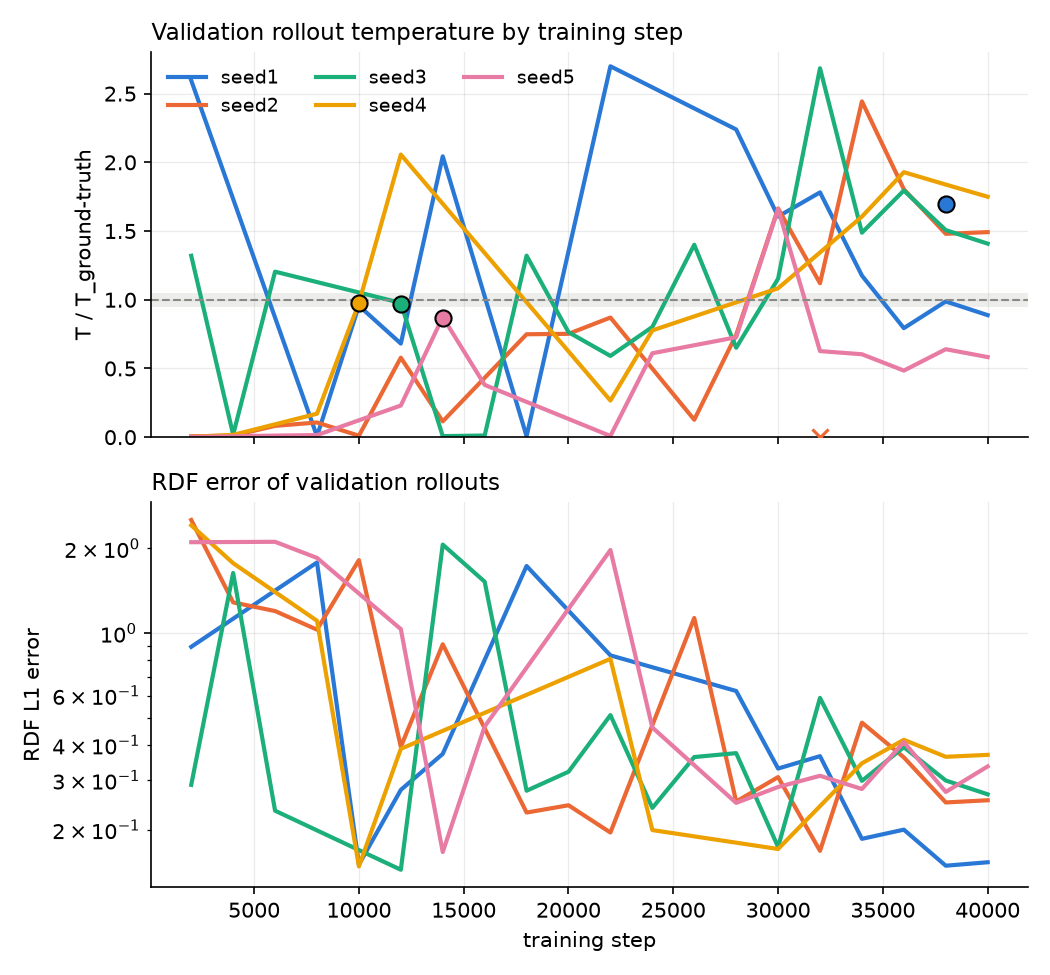
\includegraphics[width=0.8\linewidth]{../results/argon/stability_vs_step.png}
\caption{Validation rollout temperature by training step, one line per seed (argon, flow head, residual targets).}\label{fig:step}
\end{figure}

\section{Limitations}
Periodic boxes break global rotation symmetry. The model has no Hamiltonian and no energy conservation. Classical MD is faster than the model on these systems.
Argon is an easy system. Seeds are few relative to the variance we report.

\section{Related work}
TrajCast, FlashMD, Timewarp, ITO, TITO, MDGen (see docs/related\_work.md).

\end{document}
